%
% partabl.tex
%
% (c) 2024 Prof Dr Andreas Müller
%
\begin{figure}
\centering
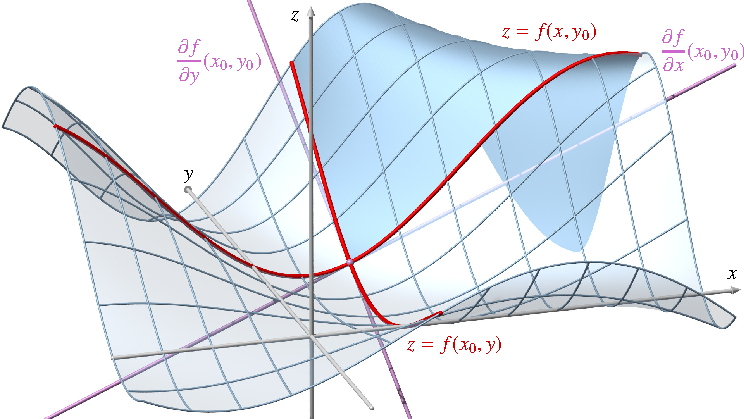
\includegraphics{chapters/010-fuvar/images/partabl.pdf}
\definecolor{tangentenfarbe}{rgb}{0.8,0.4,0.8}
\caption{Die partiellen Ableitungen einer Funktion $f(x,y)$
von Beispiel~\ref{buch:fuvar:richtungsableitung:beispiel:sincos} von
zwei Variablen im Punkt $(x_0,y_0)$ sind die Steigungen der
Koordinationenlinien im Punkt $(x,y)$.
Die Tangenten mit den entsprechenden Steigungen sind
{\color{tangentenfarbe}lila} eingezeichnet.
Die Koordinatenlinien sind die {\color{darkred}roten} Graphen der
partiellen Funktionen $x\mapsto f(x,y_0)$ und $y\mapsto f(x_0,y)$.
\label{buch:fuvar:richtungsableitung:fig:partabl}}
\end{figure}
